\section{Used Technologies}
\label{used-technologies}
In this section we will describe and explain the main technologies used in this work.

\subsection{Web Service}
Web Services are a means to enable the interoperability among application components over the Internet.  They are defined as a set of W3C standards, normally using HTTP for the transport layer and XML serialization for data interchange.

They are  a fundamental components of a programming model called Service Oriented Architecture (SOA). In this model, services are self-describing and self-contained, leading to the development of distributed systems based on loosely-coupled distributed modules.

\paragraph{Interoperability.}
Web services are not executed on client's side, so they are platform independent; they use XML for the data interchange, which is language independent; last but not the least, they use open standards, easing the integration with others components.

\paragraph{Reusable application-components.}
There are things applications need very often. So why make these over and over again? Web services can offer application-components like: currency conversion, weather reports, or even language translation as services.  [\citet{WST}]

\paragraph{Connect existing software.}
Web services can help to solve the interoperability problem between legacy and new software by giving different applications a way to link their data. With Web services one can exchange data between different applications and different platforms. [\citet{WST}]

\subsubsection{Technologies}

\paragraph{Extensible Markup Language (XML)}
is a set of rules for encoding documents in machine-readable form. It is defined in the XML 1.0 Specification produced by the W3C, and several other related specifications. It provides a language that can be used across different platforms and programming languages, and still express complex messages and functions.

\paragraph{Hypertext Transfer Protocol (HTTP)} 
is an application-level protocol for distributed, collaborative, hypermedia information systems. It is a generic, stateless, protocol which can be used for many tasks beyond its use for hypertext, such as name servers and distributed object management systems, through extension of its request methods, error codes and headers. A feature of HTTP is the typing and negotiation of data representation, allowing systems to be built independently of the data being transferred. [\citet{HTTP}]

\paragraph{Web Service Description Language (WSDL)}
is an XML format for describing services as a set of endpoints operating on messages containing either document-oriented or procedure-oriented information. The operations and messages are described abstractly, and then bound to a concrete network protocol and message format to define an endpoint. Related concrete endpoints are combined into abstract endpoints (services). WSDL is extensible to allow the description of endpoints and their messages regardless of what message formats or network protocols are used to communicate. [\citet{WSDL}]

\paragraph{Simple Object Access Protocol (SOAP)}
is a lightweight protocol for exchange of information in a decentralized, distributed environment. It is an XML based protocol that consists of three parts: an envelope that defines a framework for describing what is in a message and how to process it, a set of encoding rules for expressing instances of application-defined datatypes, and a convention for representing remote procedure calls and responses. SOAP can potentially be used in combination with a variety of other protocols; however, the only bindings in it's definition describe how to use SOAP in combination with HTTP and HTTP Extension Framework. It does not itself define any application semantics such as a programming model or implementation specific semantics; rather it defines a simple mechanism for expressing application semantics by providing a modular packaging model and encoding mechanisms for encoding data within modules. This allows SOAP to be used in a large variety of systems ranging from messaging systems to RPC.[\citet{SOAP}]

\subsection{Orchestration}
Orchestration describes how web services can interact with each other at the message level, including the business logic and execution order of the interactions. These interactions may span applications and/or organizations, resulting in a long-lived, transactional, multi-step process model. In this model of service composition, there is a central node that controls the logic of the entire process. This node has the responsibility to manage the process, choosing which services will be invoked, how messages are exchanged between these services and how to proceed with the possible exceptions and failures. Figure \ref{BPELexample} shows the message exchange between a client, a travel agency (the central node) and two web services.

\begin{figure}[htb]
  \centering
  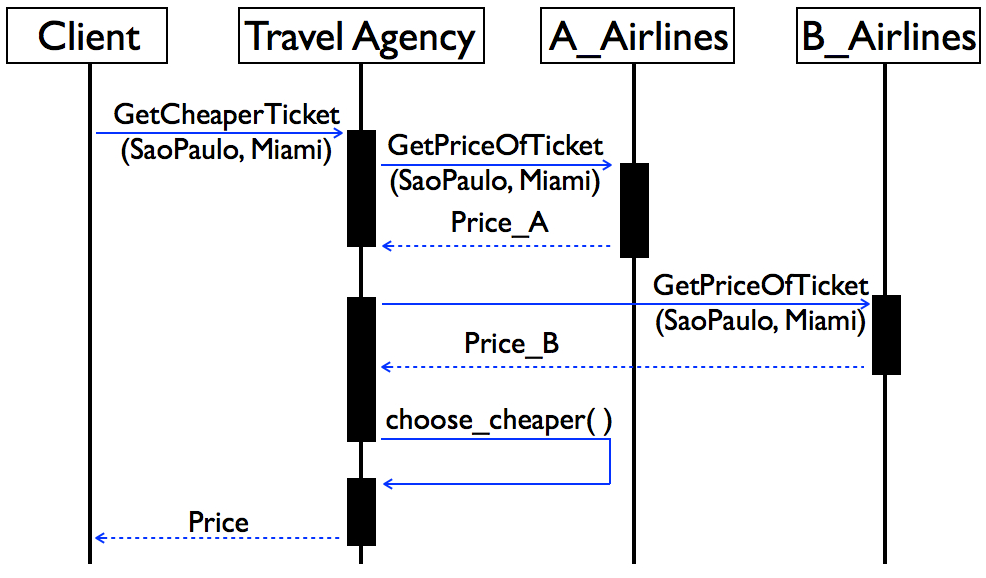
\includegraphics[width=0.9\textwidth]{images/BPELexample}
  \caption{Web Service Orchestrations example flow}
  \label{BPELexample}
\end{figure}

Basically, one must first describes the orchestration through an XML document, then generate an executable process from this file, and finally execute the process. A good analogy would be a \emph{C} program, with only the \emph{main} function (orchestration definition) that uses a lot of functions (operations) of included libraries (partner web services). The whole logic is embedded in this one description, the central node. 

The industry is embracing orchestration as the way to specify, generate and control business processes built upon web services. The acceptation of the industry came from the effort of the cooperation among companies, such as IBM, Microsoft, Sun, BEA, and others interested on the development of the Web, to standardize compositions technics. From this effort, arose these three standards candidates:

\paragraph{BPEL4WS} 
stands for ``Business Process Execution Language for Web Services''; this specification — called BPEL, for short — models the behavior of Web services in a business process interaction. It provides an XML-based grammar for describing the control logic required to coordinate Web services participating in a process flow. WSDL interfaces define the specific operations allowed and BPEL defines how to sequence them. In this sense, BPEL works as is a layer on top of WSDL. WSDL describes the public entry and exit points for every BPEL process, and WSDL data types describe the information that passes between process requests. Additionally, WSDL can reference external services that the BPEL process requires. A simple BPEL model is shown at Figure \ref{BPELstructure}.

\begin{figure}[htb]
  \centering
  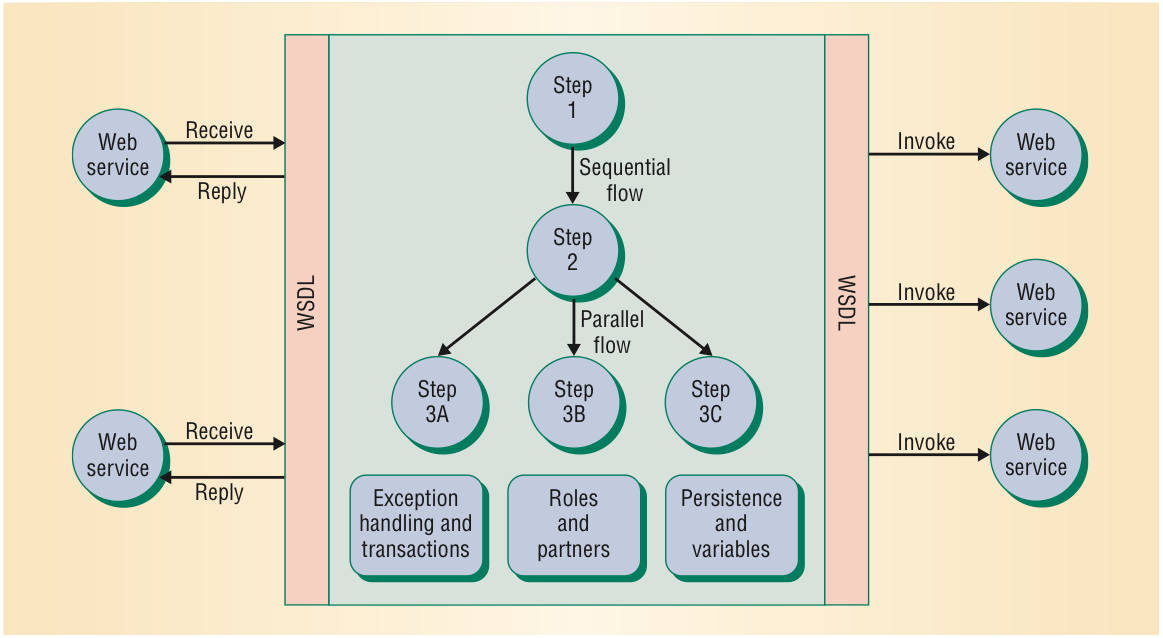
\includegraphics[width=\textwidth]{images/BPELstructure}
  \caption{BPEL structure [\citet{WSOC}]}
  \label{BPELstructure}
\end{figure}

\paragraph{WSCI}
is the ``Web Service Choreography Interface''. It is an XML-based interface description language that describes the flow of messages exchanged by a Web Service participating in choreographed interactions with other services. It describes the dynamic interface of the Web Service participating in a given message exchange by means of reusing the operations defined for a static interface. WSCI works in conjunction with the Web Service Description Language (WSDL). [\citet{WSCI}]

\paragraph{BPML} 
the ``Business Process Modeling Language'' was designed to be semantically complete according to the Pi-calculus formal representation of computational processes. In this sense it is a superset of BPEL. But, because it's formality, companies as IBM and Microsoft could not implement BPML in their existing workflow and integration engine implementations (BizTalk, Websphere etc.). Hence, they pushed for a simpler language.

In the beginning of 2003, all the companies supporting BPML discontinued it's support, migrating to BPEL4WS. It became a standard by OASIS, which renamed the standard to ``WS-BPEL'', the change was made to align with other Web Services standards of the organization. [\citet{OASIS}]

Nowadays the main standard is still BPEL, since it's definition, a lot of graphical tools, proprietary and open source softwares, were created to write it's definition. But even though there is a lot of good tools for modeling the process (e.g., NetBeans, Eclipse, Petals studio, Orchestra, and many others), there are not so many good tools for it's deployment.

\subsubsection{Tools}

\paragraph{Eclipse}
is the Rich Client Platform behind one of the most popular Java IDE in the market, the JDT. It's plugin architecture allows it to become an IDE for anything. With the BPEL Designer plugin, Eclipse enhances the ability to display and edit BPEL workflows with a graphical UI.

\paragraph{NetBeans.}
Like Eclipse, netbeans is originally a Java IDE supporting plugins. The Enterprise Edition version 6.5 brought a bundle to support the development of Web Services and Orchestrations. This was another graphical designer for BPEL, but the code it produced was readable and editable by human beings, so we used this to generate the base orchestration to the generator. NetBeans has also a module to execute the process, but it required, as mentioned before, a GUI.

\paragraph{Apache ODE}
is a WS-BPEL-compliant web services orchestration engine. It organizes web service calls following a process description written in BPEL. Another way to describe it would be a web service-capable workflow engine. This engine is the most used open source engine for orchestration available, but apache's license is not compatible with GPL, so we preferred to search other tool before using it.

\paragraph{Orchestra}
is another open source BPEL engine. It's license is LGPL, compatible with ours, but we could not find an easy way to deploy the services there.

\paragraph{PEtALS ESB}
is an Open Source Enterprise Service Bus for large SOA, Service-Oriented Architecture, architectures. [\citet{PEtALS}] An ESB is a tool that integrates existing services or applications, exposed to the Bus as a service, using standard service languages resulting in greater adaptability and automation. PEtALS ESB also has a module for executing BPEL. This way we would be able to create synthetical services in each node of the Bus and execute the composition on the Amazon Elastic Compute Cloud (Amazon EC2).


\subsection{Choreography}
Web Service Choreography is a form of service composition in which there is no single node that controls the entire process, i.e., control is distributed throughout the system. In a choreography, the interaction protocol among several partner services is defined from a global perspective. At run-time, each participant in a choreography performs a role and interacts with its neighboring participants. As there is no single point of control, and therefore, no single point of failure, there is a better potential for building scalable systems than in the case of centralized orchestrations.

The name of the composition came from the analogy of the process with dancers. While in an orchestra there is the Conductor that sets the timing and rhythm, in a group of dancers there is no coordinator during the enactment, dancers only interact with their neighbors to perform their roles.

There have been a few attempts to create standards:

\paragraph{WS-CDL}
stands for ``Web Services Choreography Description Language''; it is a W3C candidate recommendation. It is a language for describing how peer-to-peer participants collaborate. The language uses XML, and some aspects are inspired by pi-calculus

\paragraph{WSCI}
as mentioned earlier, defines a collaboration extension to WSDL, describing only the observable behavior between Web services. It does not address the definition of executables business processes.

\paragraph{BPMN}
``Business Process Modeling Notation'' is a graphical representation defined by the Object Management Group (OMG) for specifying business processes in a business process model. The new version (2.0), still in beta phase, has a set of construct blocks to specify choreography processes. This new version will also have execution semantics, which will enable the future development of tools to enact choreographies.

Although there was attempts by the W3C and OMG to specify standard languages to define choreographies, up to the moment there are no implementations that allow the enactment of choreographies specified in standard languages.

\subsection{Orchestrations versus Choreographies}

\begin{quotation}
	``Orchestration refers to an executable business process that can interact with both internal and external Web services. The interactions occur at the message level. They include business logic and task execution order, and they can span applications and organizations to define a long-lived, transactional, multi-step process model.

	Orchestration always represents control from one party’s perspective. This differs from choreography, which is more collaborative and allows each involved party to describe its part in the interaction. Choreography tracks the message sequences among multiple parties and sources —-- typically the public message exchanges that occur between Web services --- rather than a specific business process that a single party executes.'' [\citet{WSOC}]
\end{quotation}

A graphical view of the relationship described by Peltz is represented in Figure \ref{relation-orchestrationXchoreography}.

\begin{figure}[htb]
	\centering
	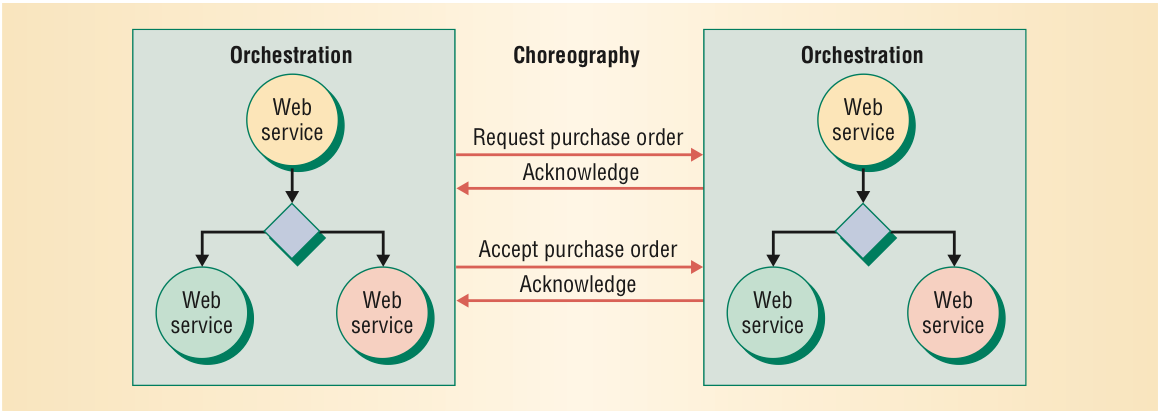
\includegraphics[width=\textwidth]{images/relation-orchestrationXchoreography}
	\caption{Relationship between Orchestrations and Choreographies [\citet{WSOC}]}
	\label{relation-orchestrationXchoreography}
\end{figure}




\subsection{Cloud Computing}
More recently, a new generation of middleware systems and hardware infrastructures were developed to cope with other kinds of applications requiring large processing power. In this case, the motivation was end-user applications such as email, office suites, calendars, and many other e-commerce, social networks, and Web 2.0-style applications used daily by hundreds of millions of users. Large Internet-based companies such as Amazon and Google used virtualization technologies to develop the basis for what was later called Cloud Computing [\citet{ZCB10}]. Google App Engine provides an execution environment for Web applications that can then be executed in the hardware infrastructure provided by Google; developers can write applications in Java or Python and use standard APIs for storage and communication.  The Amazon Elastic Compute Cloud or EC2 [\citet{EC2}] provides a virtual computing environment in which developers can instantiate multiple virtual machines booting, from scratch, standard operating systems such as GNU/Linux or Windows. These sets of machines can then run any application developed for these operating systems. When necessary, the developer can also create an image from a current instance of his virtual machines set and then create new instances with the given image, shortening the configuration time for these new machines.

Cloud computing brought an ease of deployment and scalability never seen before. With Amazon's service, one can ensure that the number of Amazon EC2 instances one is using scales up seamlessly during demand spikes to maintain performance, and scales down automatically during demand lulls to minimize costs, using pre-defined rules based upon CPU, RAM and Network usage. Also, it is trivial to, for example, build scripts to scale the service up at a certain time and later scale it down over the dawn, when there might be less people accessing the service. [\citet{AUTO-SCALE}]

